\chapter{Bằng chứng, thực thi và tái hiện}\label{app:evidence}
\section{Nguồn bằng chứng và môi trường}
Năm notebook giữ source và output thực nghiệm. Dataset dùng 20 Parquet và bốn JSON xác minh; PhoBERT dùng \texttt{result/evaluation/}, ba đối chứng dùng \texttt{result/<model>/evaluation/} với \texttt{<model>} là svm, logistic hoặc lstm. Metrics và config chọn liên kết số tổng với classification report, ma trận và dự đoán từng bài. \texttt{split\_manifest.json} cùng \texttt{article\_metadata.parquet} xác định đúng thứ tự mẫu, không chỉ số lượng.

Metadata PhoBERT ghi Python 3.14.7, PyTorch 2.11.0+cu128, CUDA 12.8, Transformers 5.17.0, NumPy 2.5.2, pandas 3.0.6, scikit-learn 1.9.1, PyArrow 26.0.0 và PyVi 0.1.1. Neural dùng RTX A3000 Laptop 12 GB; các notebook đối chứng ghi CPU/GPU cùng phạm vi timer riêng. Đổi phiên bản, kernel hoặc precision có thể làm thay đổi tốc độ và điểm số sát ranh giới.

\section{Tái hiện và đối chiếu integrity}
Đọc output và các file evaluation cho phép kiểm tra kết quả mà không train lại. Scores/logits và predictions được tái tính để xác nhận Accuracy, F1, support; tổng mỗi ma trận bằng 29.995. Mảng split của bốn model giống nhau, toàn bộ URL/nhãn test khớp theo thứ tự; chuỗi signature có thể khác vì cách tạo hash khác nhau. Các label mapping và calibration phải được đối chiếu cùng checkpoint thay vì nạp một tokenizer bất kỳ.

Với dataset đã khóa, mỗi notebook model thực thi độc lập. Fresh tạo lượt mới; evaluate cần artifact tương thích. Continue của BiLSTM/PhoBERT nạp trọng số tương thích nhưng khởi tạo lại optimizer/scheduler, không resume trạng thái giữa epoch. Crawl lại có thể đổi snapshot vì HTML và phạm vi xuất bản thay đổi. README chứa lệnh vận hành và đường dẫn chi tiết.

Gói active của app có SHA trọng số bắt đầu \texttt{607f3240}; mapping, Head--Tail, tiền xử lý và calibration khớp gói PhoBERT. SHA xác nhận đúng byte của artifact, không xác nhận nhãn ngữ nghĩa của mọi bài. Các đồ thị ghép panel trong báo cáo dùng cùng số liệu nguồn; ma trận 20 lớp vẫn hiển thị riêng để giữ khả năng đọc. Đường PR từng lớp, history chi tiết và các chẩn đoán khác được giữ ở assets/output notebook, không cần đưa toàn bộ vào PDF.
\clearpage
\section{Ma trận chuẩn hóa các đối chứng}
Ba hình dùng cùng ID ở bảng~\ref{tab:class_split}, đơn vị phần trăm theo support hàng. Đối chiếu với ma trận PhoBERT cần đổi thang 0--1 thành phần trăm; không so màu mà bỏ qua đơn vị.
\begin{figure}[htbp]\centering
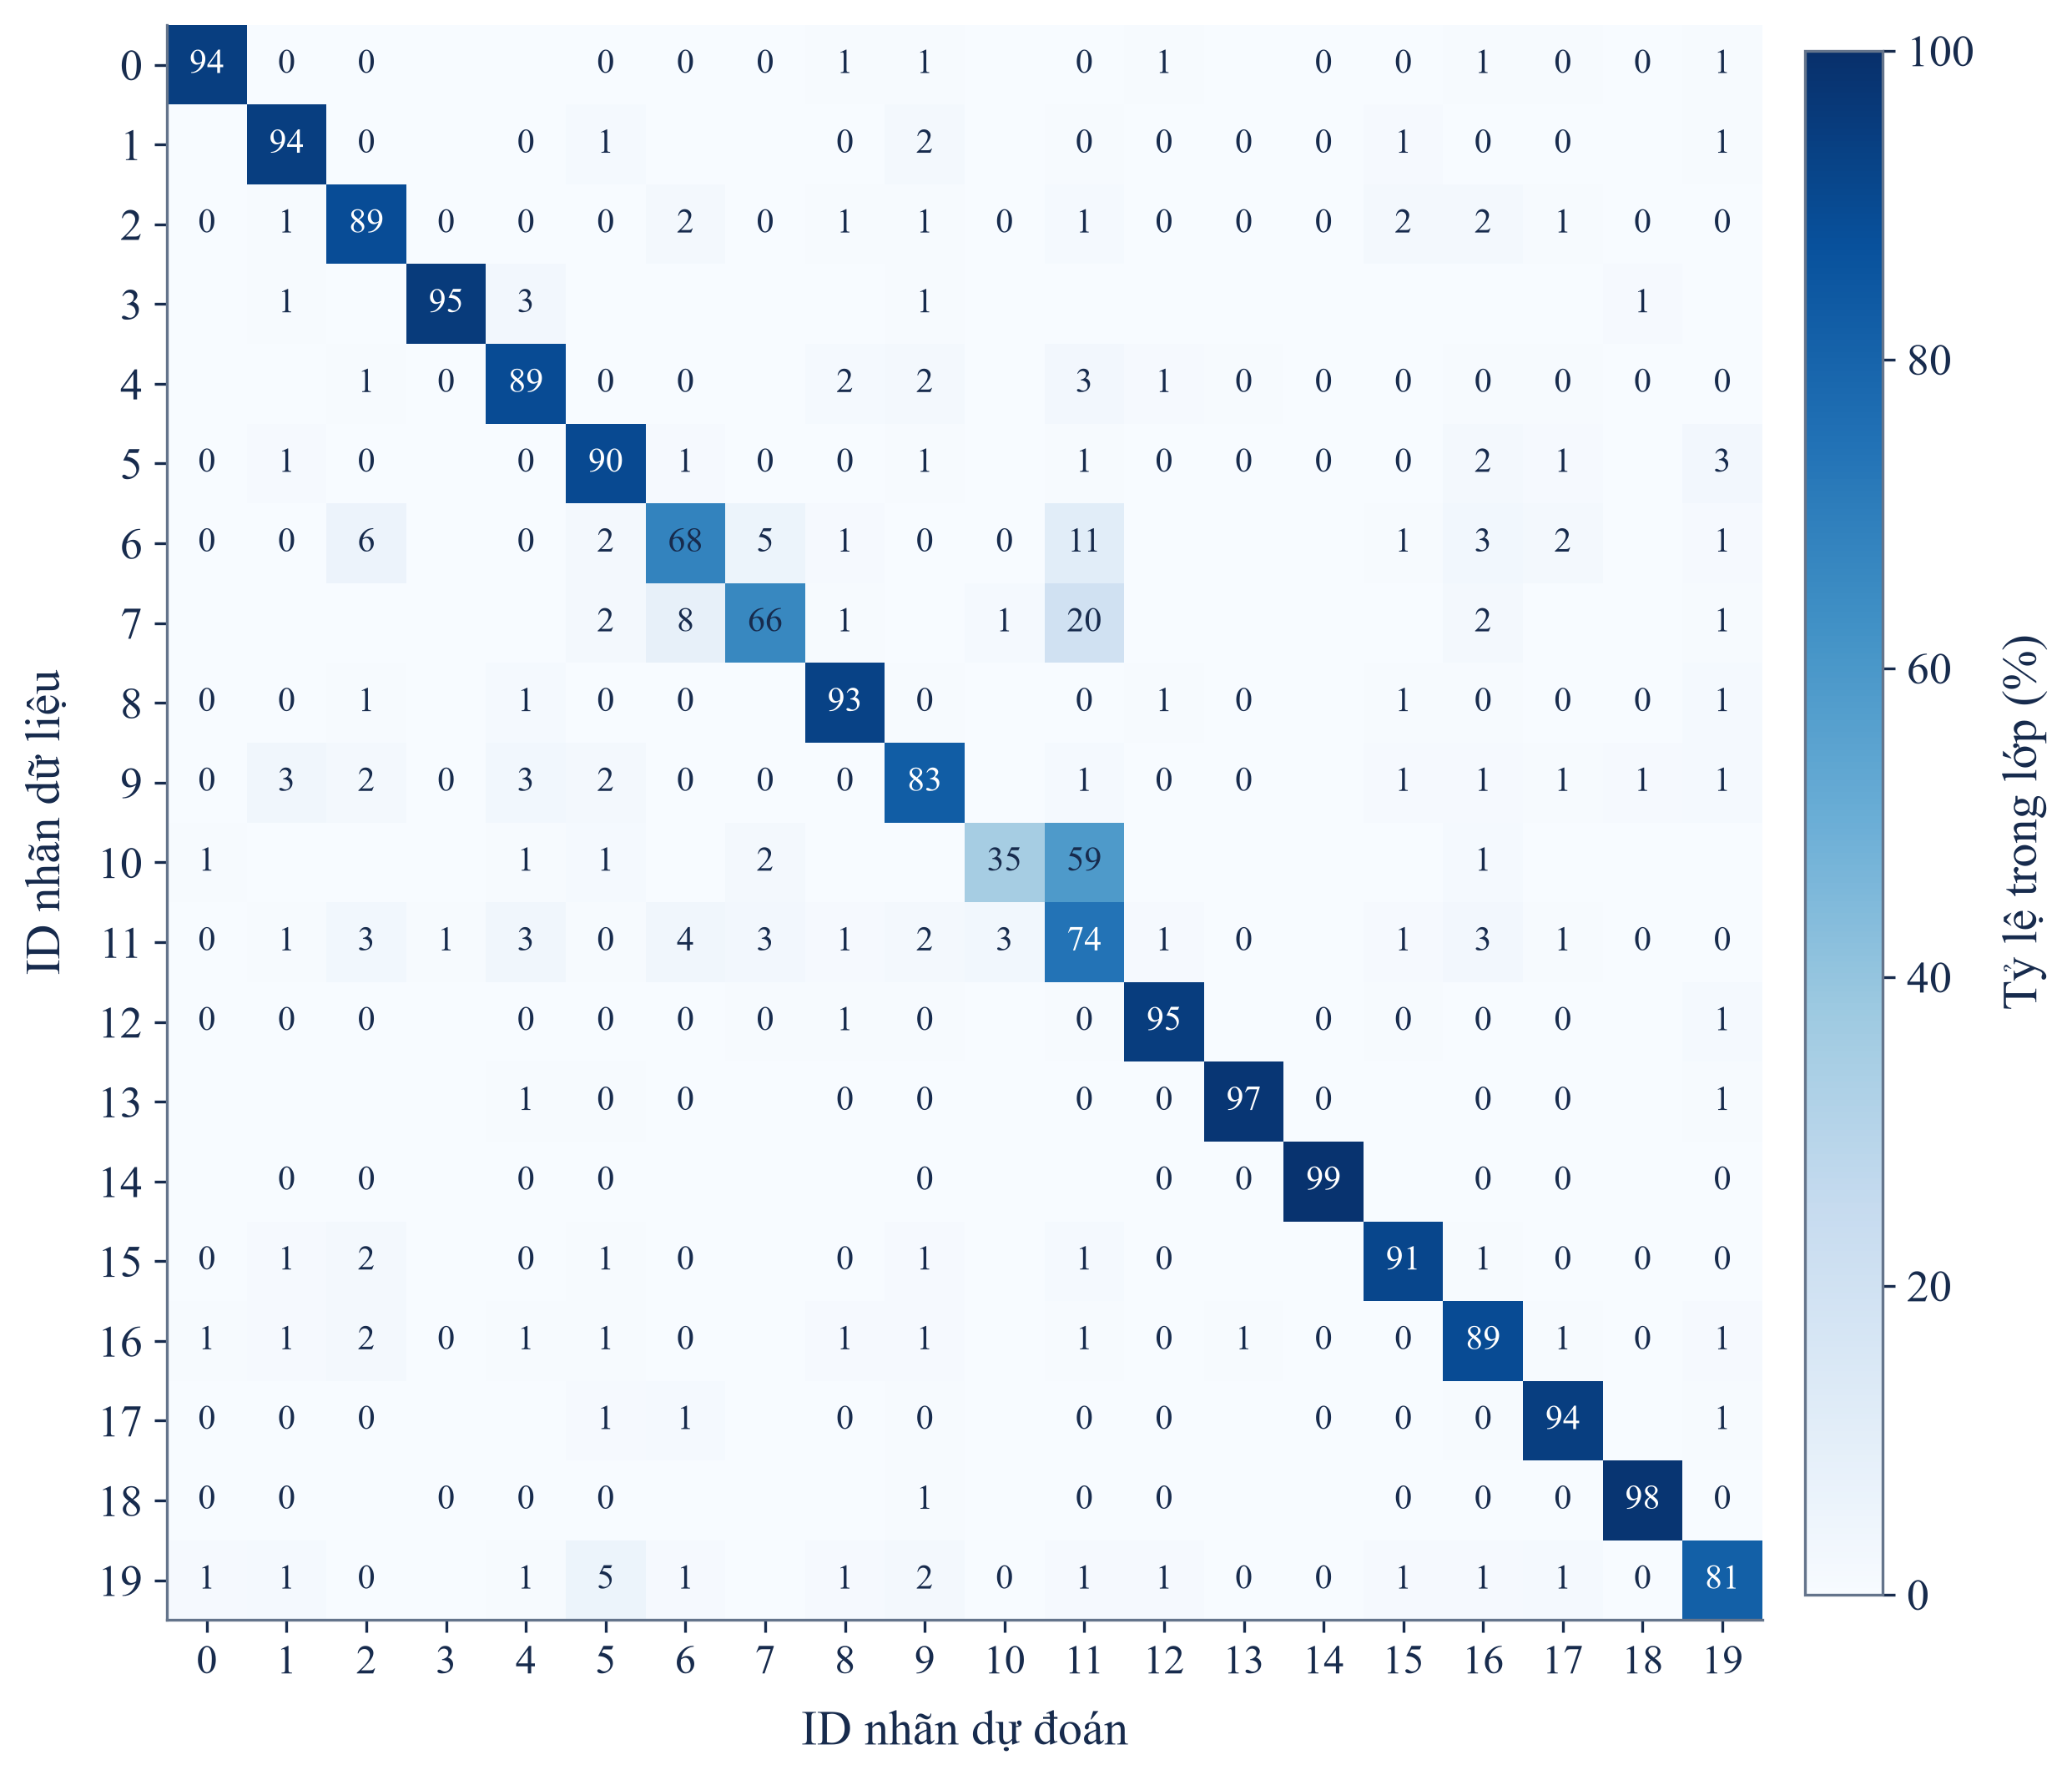
\includegraphics[width=.96\textwidth,height=.70\textheight,keepaspectratio]{assets/baselines/svm/evaluation/confusion_matrix_normalized.png}
\caption{Linear SVM, argmax trên 29.995 bài test; chuẩn hóa theo hàng (\%).}\end{figure}
\clearpage
\begin{figure}[htbp]\centering
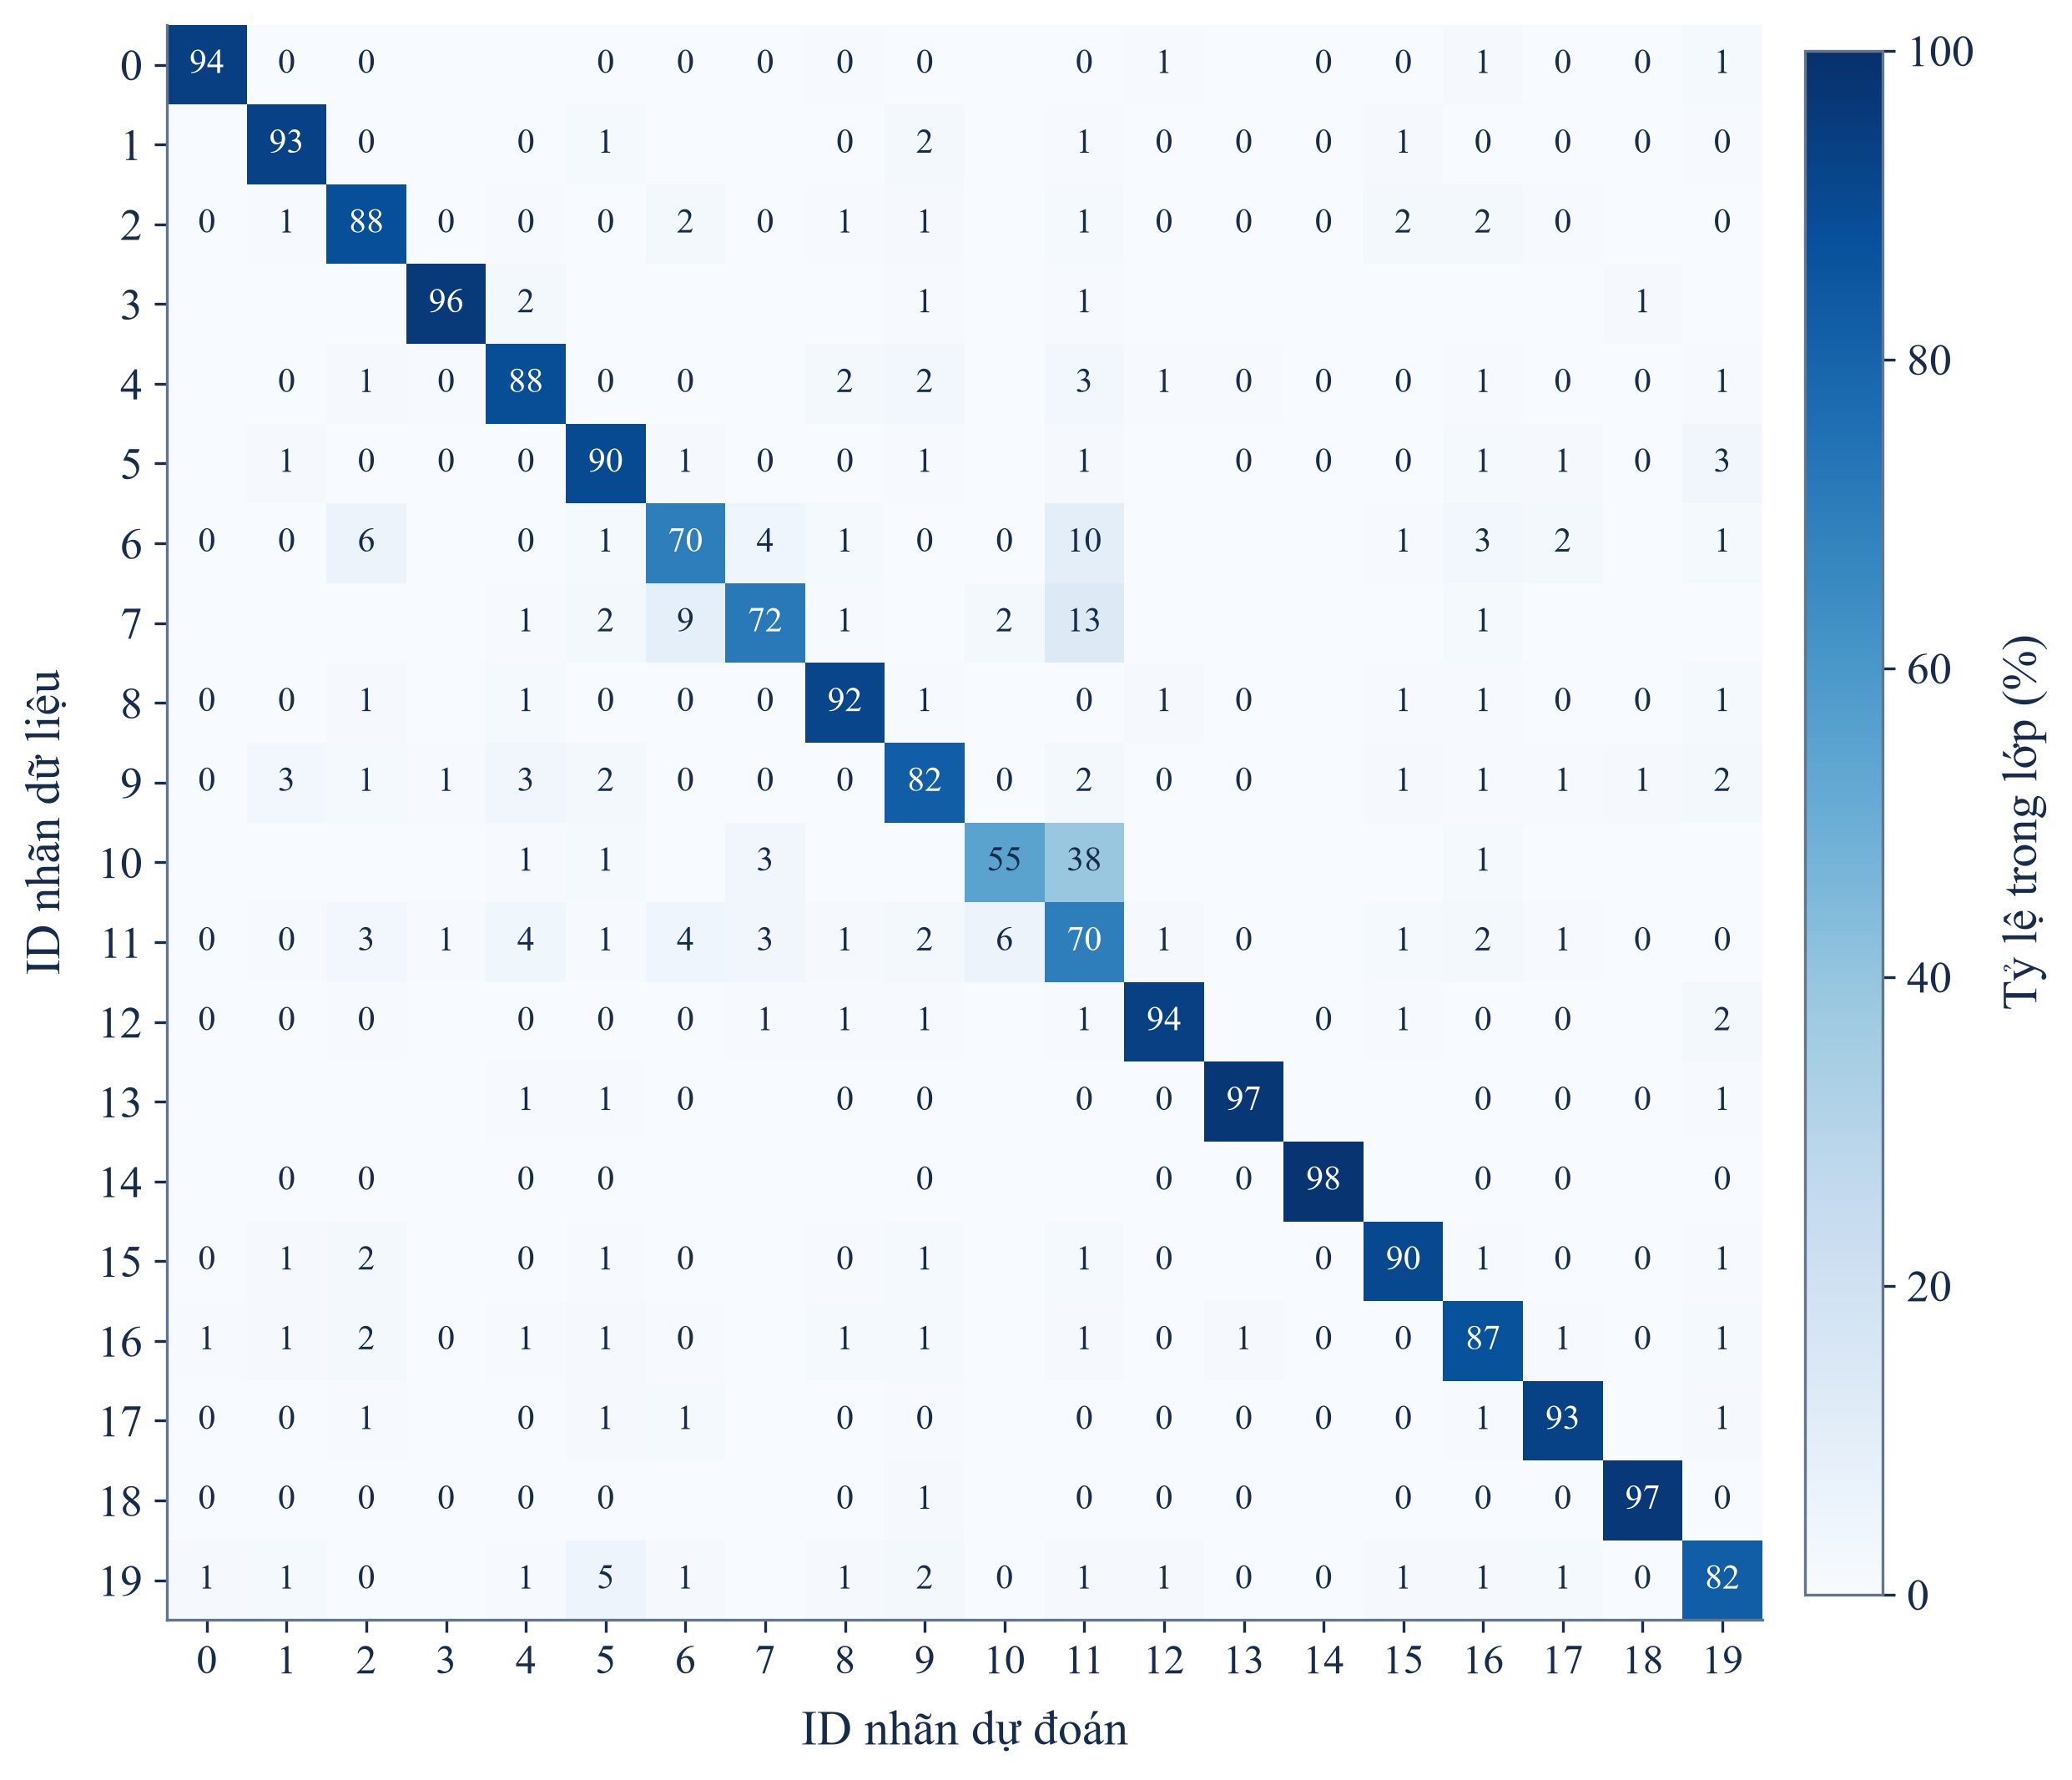
\includegraphics[width=.96\textwidth,height=.74\textheight,keepaspectratio]{assets/baselines/logistic/evaluation/confusion_matrix_normalized.png}
\caption{Logistic Regression, cùng test và taxonomy; chuẩn hóa theo hàng (\%).}\end{figure}
\clearpage
\begin{figure}[htbp]\centering
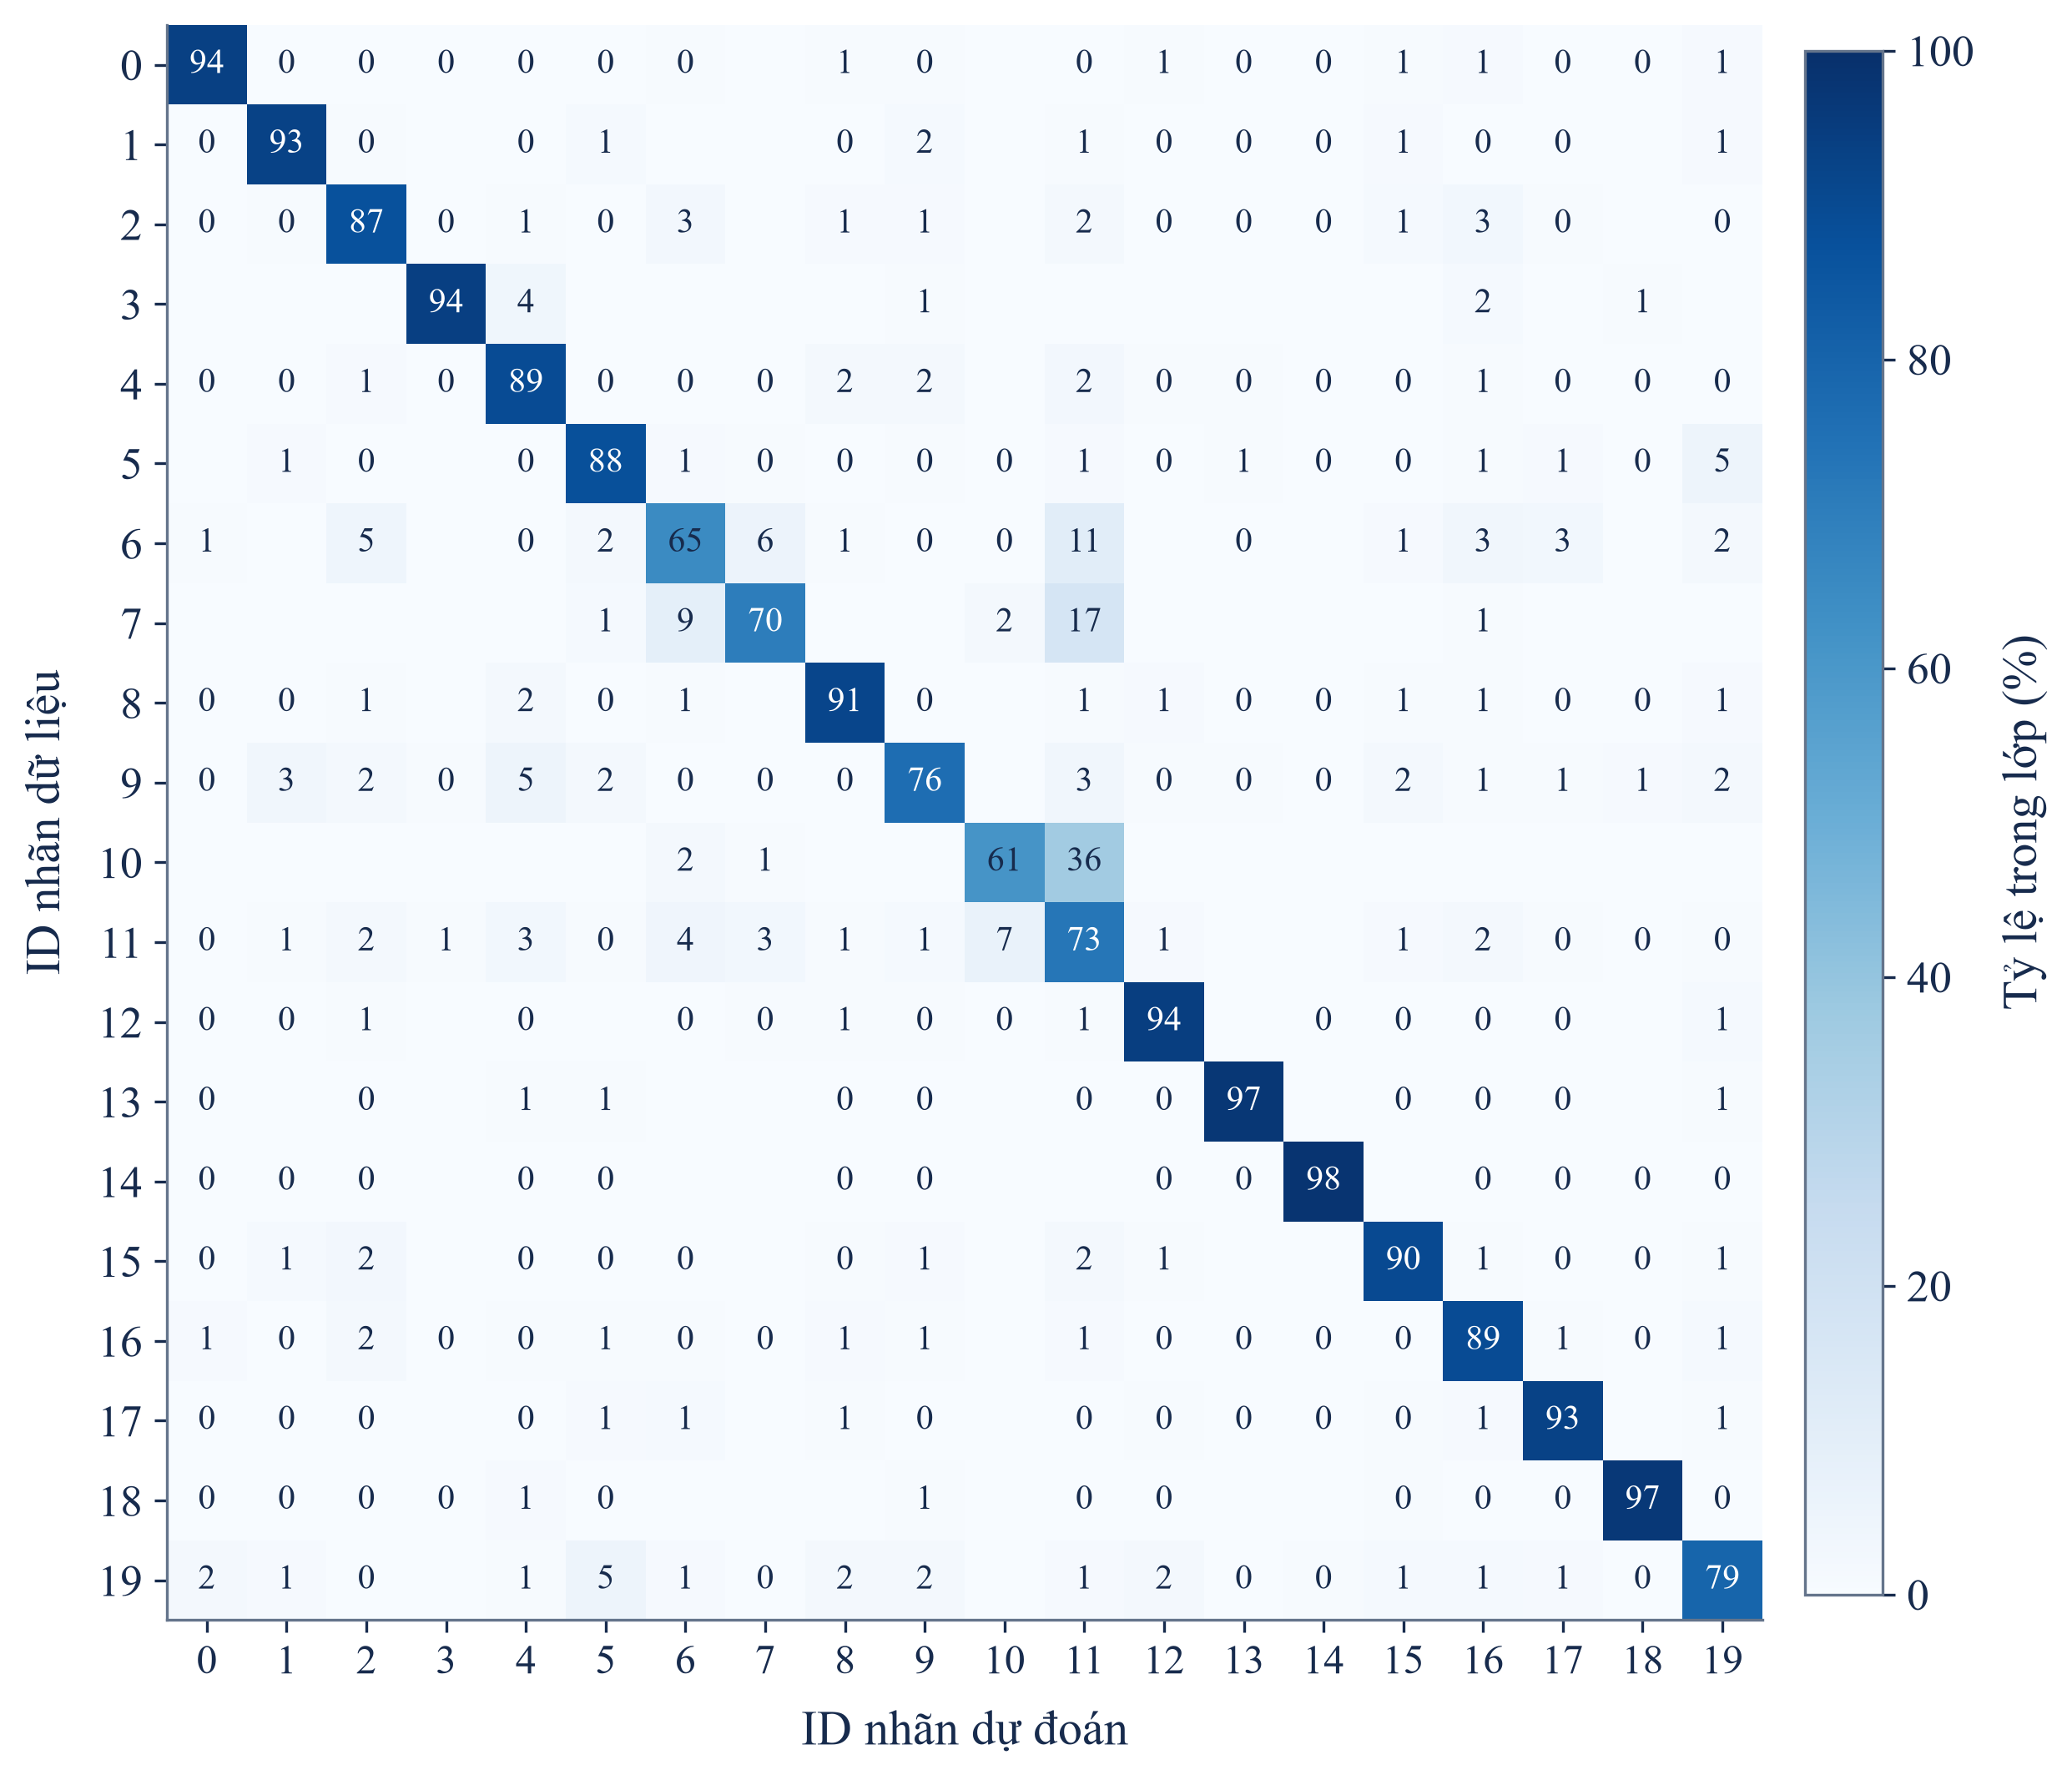
\includegraphics[width=.96\textwidth,height=.74\textheight,keepaspectratio]{assets/baselines/lstm/evaluation/confusion_matrix_normalized.png}
\caption{BiLSTM, cùng test và taxonomy; chuẩn hóa theo hàng (\%).}\end{figure}
